\clearpage
\cleardoublepage

\chapter{神经网络架构}

\section{引言}

神经网络架构定义了神经元的组织方式和连接方式，以处理信息。不同的架构适用于不同类型的数据和任务。本章涵盖三种基本神经网络架构：深度神经网络（DNN）、卷积神经网络（CNN）和循环神经网络（RNN）。

\section{深度神经网络（DNN）}

深度神经网络由多层神经元组成，信息从输入流向输出，没有循环。

\subsection{架构}

全连接 DNN 执行：
\begin{equation}
\mathbf{h}^{(l)} = f^{(l)}(\mathbf{W}^{(l)}\mathbf{h}^{(l-1)} + \mathbf{b}^{(l)})
\end{equation}
其中 $l = 1, \ldots, L$ 是层的索引。

\begin{figure}[htbp]
    \centering
    \begin{tikzpicture}[scale=0.8]
        % 输入层
        \foreach \y in {1,...,4} {
            \node[circle, draw=layer-input, fill=layer-input!30] (i\y) at (0, 5-\y) {};
        }
        \node[below] at (0, 0.5) {输入层};
        
        % 隐藏层1
        \foreach \y in {1,...,5} {
            \node[circle, draw=layer-hidden, fill=layer-hidden!30] (h1\y) at (3, 5.5-\y) {};
        }
        
        % 隐藏层2
        \foreach \y in {1,...,4} {
            \node[circle, draw=layer-hidden, fill=layer-hidden!30] (h2\y) at (6, 5-\y) {};
        }
        
        % 输出层
        \foreach \y in {1,...,2} {
            \node[circle, draw=layer-output, fill=layer-output!30] (o\y) at (9, 4.5-\y) {};
        }
        \node[below] at (9, 2) {输出层};
        
        % 连接（采样）
        \foreach \i in {1,...,4} {
            \foreach \j in {1,...,5} {
                \draw[gray, opacity=0.2] (i\i) -- (h1\j);
            }
        }
        \foreach \i in {1,...,5} {
            \foreach \j in {1,...,4} {
                \draw[gray, opacity=0.2] (h1\i) -- (h2\j);
            }
        }
        \foreach \i in {1,...,4} {
            \foreach \j in {1,...,2} {
                \draw[gray, opacity=0.2] (h2\i) -- (o\j);
            }
        }
    \end{tikzpicture}
    \caption{深度神经网络架构}
    \label{fig:dnn}
\end{figure}

\begin{properties}[DNN特性]
\begin{itemize}
    \item \textbf{参数量：}$\sum_{l=1}^{L} (n^{(l-1)} \cdot n^{(l)} + n^{(l)})$
    \item \textbf{通用逼近：}在足够宽度/深度下可以逼近任何连续函数
    \item \textbf{适用于：}表格数据、基于特征的分类
\end{itemize}
\end{properties}

\section{卷积神经网络（CNN）}

CNN 通过局部连接和参数共享来利用数据的空间结构。

\subsection{卷积层}

卷积操作：
\begin{equation}
y[i,j] = \sum_{m}\sum_{n} w[m,n] \cdot x[i+m, j+n]
\end{equation}

\begin{figure}[htbp]
    \centering
    \begin{tikzpicture}[scale=0.7]
        % 输入特征图
        \foreach \x in {0,...,3} {
            \foreach \y in {0,...,3} {
                \fill[blue!30] (\x, \y) +(-0.4, -0.4) rectangle ++(0.4, 0.4);
            }
        }
        \node at (1.5, -1) {输入特征图};
        
        % 卷积核
        \foreach \x in {0,...,2} {
            \foreach \y in {0,...,2} {
                \fill[red!30] (5+\x, 1+\y) +(-0.4, -0.4) rectangle ++(0.4, 0.4);
            }
        }
        \node at (6.5, -1) {卷积核 $3 \times 3$};
        
        % 输出
        \foreach \x in {0,...,1} {
            \foreach \y in {0,...,1} {
                \fill[green!30] (10+\x, 0.5+\y) +(-0.4, -0.4) rectangle ++(0.4, 0.4);
            }
        }
        \node at (10.5, -1) {输出 $2 \times 2$};
        
        % 箭头
        \draw[->, thick] (4, 1.5) -- (4.5, 1.5);
        \draw[->, thick] (8.5, 1.5) -- (9.5, 1.5);
    \end{tikzpicture}
    \caption{卷积操作}
    \label{fig:convolution}
\end{figure}

关键参数：
\begin{itemize}
    \item \textbf{卷积核大小：}$K \times K$（通常 $3 \times 3$、$5 \times 5$、$7 \times 7$）
    \item \textbf{步长：}$s$（步长大小，通常1或2）
    \item \textbf{填充：}$p$（用于控制输出大小的零填充）
\end{itemize}

输出尺寸：
\begin{equation}
H_{out} = \left\lfloor \frac{H_{in} + 2p - K}{s} + 1 \right\rfloor
\end{equation}

\begin{properties}[CNN优势]
\begin{itemize}
    \item \textbf{局部感受野：}每个神经元只看到局部区域
    \item \textbf{参数共享：}跨空间位置使用相同权重
    \item \textbf{平移等变性：}输入移位 $\rightarrow$ 输出移位
    \item \textbf{适用于：}图像、视频、空间数据
\end{itemize}
\end{properties}

\subsection{感受野分析}

\textbf{感受野}（RF）是影响其输出的输入图像区域。理解感受野增长对架构设计至关重要。

\subsubsection{单层感受野}

具有卷积核 $K$、步长 $s$ 和填充 $p$ 的单层卷积产生的输出感受野就是 $K$。输出尺寸为：
\begin{equation}
o_i = \left\lfloor \frac{i_{in} + 2p - K}{s} + 1 \right\rfloor
\end{equation}

\subsubsection{多层感受野}

对于 $L$ 层卷积堆叠，输出的有效感受野（ERF）增长为：
\begin{equation}
\text{RF} = 1 + \sum_{l=1}^{L} \left( (K_l - 1) \cdot \prod_{l'=1}^{l-1} s_{l'} \right)
\end{equation}

\begin{example}[两个 $3 \times 3$ 卷积]
两个步长为1堆叠的 $3 \times 3$ 卷积：
\begin{equation}
\text{RF} = 1 + (3 - 1) \times 1 + (3 - 1) \times 1 = 5 \times 5
\end{equation}
这与单个 $5 \times 5$ 卷积的感受野匹配，但参数更少（$2 \times 9C^2$ vs $25C^2$）。
\end{example}

\subsubsection{有效感受野}

虽然\textbf{理论}感受野覆盖上述整个区域，但\textbf{有效}感受野（实际影响输出的区域）在感受野中心呈高斯类分布 \cite{luo2016understanding}。边界附近的像素比中心像素对输出的贡献少得多。

这有重要的设计含义：
\begin{itemize}
    \item 简单增加理论感受野不会按比例增加有效感受野
    \item 空洞/带孔卷积可以在不增加参数的情况下扩展有效感受野
    \item 相对于大卷积核的浅层网络，更偏好小卷积核的深层网络
\end{itemize}

\subsection{\texorpdfstring{$1 \times 1$}{1x1} 卷积：跨通道混合}

$1 \times 1$ 卷积，也称为\textbf{逐点卷积}，独立地对每个像素进行操作，但混合跨通道的信息。尽管简单，它是现代架构中最通用的操作之一。

\textbf{数学解释。}具有 $C_{in}$ 输入通道和 $C_{out}$ 输出通道的 $1 \times 1$ 卷积等效于在每个空间位置应用全连接层：
\begin{equation}
y_{c_{out}}[i, j] = \sum_{c_{in}=1}^{C_{in}} w_{c_{out}, c_{in}} \cdot x_{c_{in}}[i, j] + b_{c_{out}}
\end{equation}

这可以写为矩阵乘法：$\mathbf{Y}[i,j] = \mathbf{W} \cdot \mathbf{X}[i,j]$，其中 $\mathbf{W} \in \mathbb{R}^{C_{out} \times C_{in}}$。

\begin{properties}[$1 \times 1$ 卷积的关键用途]
\begin{itemize}
    \item \textbf{降维（瓶颈）：}在昂贵的 $3 \times 3$ 卷积前将 $C_{in} \to C_{in}/4$，然后投影回来。用于 Inception、ResNet 瓶颈和 MobileNet。参数：$C_{in} \times C_{out}$（vs $K^2 \times C_{in} \times C_{out}$ 的 $K \times K$ 卷积）。
    \item \textbf{通道混合：}启用跨通道信息流而不进行空间聚合。当需要不同卷积核的特征交互时必不可少。
    \item \textbf{非线性注入：}每个 $1 \times 1$ 卷积后，激活函数（ReLU/GELU）增加表示能力。在 ResNeXt 和 MLP-Mixer 中，这些"通道 MLP"被堆叠。
    \item \textbf{增加深度而不增加空间成本：}增加网络深度而不影响空间分辨率或显著增加参数。
\end{itemize}
\end{properties}

\subsection{转置卷积（反卷积）}

对于上采样任务（分割、生成），\textbf{转置卷积}（有时称为反卷积）反转标准卷积的空间缩减。

给定由步长 $s$、填充 $p$ 和卷积核 $K$ 定义的卷积，转置卷积将输入尺寸 $H_{in}$ 映射到：
\begin{equation}
H_{out} = (H_{in} - 1) \times s - 2p + K
\end{equation}

\begin{note}[转置卷积 $\neq$ 逆卷积]
转置卷积\textbf{不是}卷积的数学逆。它是卷积算子的转置（因此得名）。给定 $\mathbf{Y} = \mathbf{C}\mathbf{X}$ 其中 $\mathbf{C}$ 是作为矩阵的卷积，转置卷积计算 $\mathbf{C}^\top \mathbf{Y}$。这具有相同参数但不能精确恢复 $\mathbf{X}$。
\end{note}

\section{循环神经网络（RNN）}

RNN 通过维护隐藏状态来处理序列数据。

\subsection{架构}

对于输入序列 $\mathbf{x}^{(1)}, \mathbf{x}^{(2)}, \ldots, \mathbf{x}^{(T)}$：
\begin{align}
\mathbf{h}^{(t)} &= f(\mathbf{W}_{xh}\mathbf{x}^{(t)} + \mathbf{W}_{hh}\mathbf{h}^{(t-1)} + \mathbf{b}_h) \\
\mathbf{y}^{(t)} &= g(\mathbf{W}_{hy}\mathbf{h}^{(t)} + \mathbf{b}_y)
\end{align}

\begin{figure}[htbp]
    \centering
    \begin{tikzpicture}[scale=0.8]
        % RNN单元
        \node[draw, minimum width=2cm, minimum height=1.5cm, rounded corners] (rnn) at (0,0) {RNN单元};
        
        % 输入
        \node (x) at (-2, 0) {$\mathbf{x}^{(t)}$};
        \node (h_prev) at (0, 2) {$\mathbf{h}^{(t-1)}$};
        
        % 输出
        \node (h) at (0, -2) {$\mathbf{h}^{(t)}$};
        \node (y) at (2, 0) {$\mathbf{y}^{(t)}$};
        
        % 箭头
        \draw[->] (x) -- (rnn);
        \draw[->] (h_prev) -- (rnn);
        \draw[->] (rnn) -- (h);
        \draw[->] (rnn) -- (y);
        
        % 循环箭头
        \draw[->, bend left] (h) to (h_prev);
        \node[right] at (-0.3, 1.2) {循环};
    \end{tikzpicture}
    \caption{RNN架构}
    \label{fig:rnn}
\end{figure}

\begin{properties}[RNN特性]
\begin{itemize}
    \item \textbf{序列处理：}可以处理可变长度序列
    \item \textbf{共享参数：}跨时间步使用相同权重
    \item \textbf{记忆：}隐藏状态捕获过去信息
    \item \textbf{适用于：}文本、时间序列、音频、视频
\end{itemize}
\end{properties}

\begin{note}[梯度消失问题]
标准 RNN 在时间反向传播（BPTT）期间遭受梯度消失，使得学习长期依赖变得困难。这导致了 LSTM 和 GRU 架构的发展。
\end{note}

\subsection{RNN 中的梯度消失：数学证明}

理解\textbf{为什么} vanilla RNN 在长序列上失败需要检查通过时间的梯度流动。我们推导出梯度消失的精确条件。

\subsubsection{时间反向传播（BPTT）}

考虑序列长度 $T$ 上的总损失：
\begin{equation}
\mathcal{L} = \sum_{t=1}^{T} \ell(\mathbf{y}^{(t)}, \hat{\mathbf{y}}^{(t)})
\end{equation}

$\mathcal{L}$ 关于早期时间步 $k$ 的 $\mathbf{h}^{(k)}$ 的梯度涉及雅可比矩阵链：
\begin{equation}
\frac{\partial \mathcal{L}}{\partial \mathbf{h}^{(k)}} = \frac{\partial \mathcal{L}}{\partial \mathbf{h}^{(T)}} \prod_{t=k+1}^{T} \frac{\partial \mathbf{h}^{(t)}}{\partial \mathbf{h}^{(t-1)}}
\end{equation}

隐藏状态转换的雅可比矩阵（带 $\mathbf{h}^{(t)} = \tanh(\mathbf{W}_{hh}\mathbf{h}^{(t-1)} + \mathbf{W}_{xh}\mathbf{x}^{(t)} + \mathbf{b})$）为：
\begin{equation}
\frac{\partial \mathbf{h}^{(t)}}{\partial \mathbf{h}^{(t-1)}} = \text{diag}\bigl(1 - (\mathbf{h}^{(t)})^2\bigr) \cdot \mathbf{W}_{hh}
\end{equation}

\subsubsection{谱分析}

$T - k$ 个雅可比矩阵的乘积可以通过它们的谱特性来分析：
\begin{equation}
\left\| \prod_{t=k+1}^{T} \frac{\partial \mathbf{h}^{(t)}}{\partial \mathbf{h}^{(t-1)}} \right\| \leq \prod_{t=k+1}^{T} \left\| \frac{\partial \mathbf{h}^{(t)}}{\partial \mathbf{h}^{(t-1)}} \right\| \leq \prod_{t=k+1}^{T} \gamma_t
\end{equation}
其中 $\gamma_t = \lambda_{\max}\bigl(\mathbf{W}_{hh}\bigr) \cdot \sup_i |1 - (h_i^{(t)})^2| \leq \lambda_{\max}\bigl(\mathbf{W}_{hh}\bigr)$ 因为 $|1 - \tanh^2(x)| \leq 1$。

\begin{定理}[梯度消失/爆炸条件]
通过时间的梯度满足：
\begin{equation}
\left\| \frac{\partial \mathcal{L}}{\partial \mathbf{h}^{(k)}} \right\| \approx \left\| \frac{\partial \mathcal{L}}{\partial \mathbf{h}^{(T)}} \right\| \cdot \gamma^{T-k}
\end{equation}
其中 $\gamma = \lambda_{\max}(\mathbf{W}_{hh})$。因此：
\begin{itemize}
    \item 如果 $\gamma < 1$：梯度\textbf{指数消失}为 $\gamma^{T-k} \to 0$
    \item 如果 $\gamma > 1$：梯度\textbf{指数爆炸}
    \item 如果 $\gamma = 1$（在边界上）：梯度被保留，但这是一个零测度条件
\end{itemize}
\end{定理}

\begin{properties}[为什么这在实践中很重要]
\begin{itemize}
    \item 典型的随机初始化以高概率产生 $\gamma \ll 1$ \cite{bengio1994learning}
    \item 对于序列长度 $T = 100$ 和 $\gamma = 0.9$：梯度幅度 $\approx 0.9^{100} \approx 2.7 \times 10^{-5}$ —— 有效地为零
    \item $\mathbf{W}_{hh}$ 的特征值被 $\tanh$ 导数限制在 $[-1, 1]$，推向消失
    \item 这本质上是\textbf{动力系统}问题：RNN 是一个离散时间动力系统，其不动点要么是吸引的（$\gamma < 1$）要么是排斥的（$\gamma > 1$）
\end{itemize}
\end{properties}

\section{长短期记忆网络（LSTM）}

LSTM \cite{hochreiter1997long} 用门控机制解决梯度消失问题。

\subsection{LSTM门}

\begin{align}
\mathbf{f}^{(t)} &= \sigma(\mathbf{W}_f[\mathbf{h}^{(t-1)}, \mathbf{x}^{(t)}] + \mathbf{b}_f) \quad \text{(遗忘门)} \\
\mathbf{i}^{(t)} &= \sigma(\mathbf{W}_i[\mathbf{h}^{(t-1)}, \mathbf{x}^{(t)}] + \mathbf{b}_i) \quad \text{(输入门)} \\
\mathbf{o}^{(t)} &= \sigma(\mathbf{W}_o[\mathbf{h}^{(t-1)}, \mathbf{x}^{(t)}] + \mathbf{b}_o) \quad \text{(输出门)} \\
\tilde{\mathbf{c}}^{(t)} &= \tanh(\mathbf{W}_c[\mathbf{h}^{(t-1)}, \mathbf{x}^{(t)}] + \mathbf{b}_c) \quad \text{(细胞候选)} \\
\mathbf{c}^{(t)} &= \mathbf{f}^{(t)} \odot \mathbf{c}^{(t-1)} + \mathbf{i}^{(t)} \odot \tilde{\mathbf{c}}^{(t)} \quad \text{(细胞状态)} \\
\mathbf{h}^{(t)} &= \mathbf{o}^{(t)} \odot \tanh(\mathbf{c}^{(t)}) \quad \text{(隐藏状态)}
\end{align}

\begin{figure}[htbp]
    \centering
    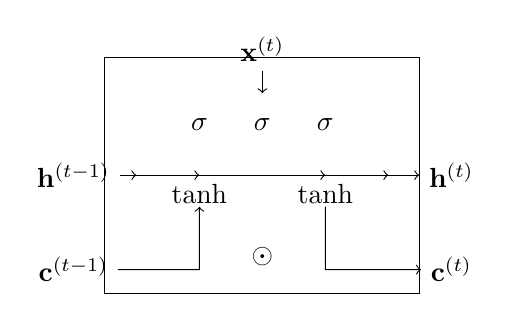
\begin{tikzpicture}[scale=0.8]
        % LSTM单元表示
        \node[draw, rectangle, minimum width=4cm, minimum height=3cm] (lstm) at (0,0) {};
        
        % 内部结构
        \node at (-1, 0.8) {$\sigma$};
        \node at (0, 0.8) {$\sigma$};
        \node at (1, 0.8) {$\sigma$};
        \node at (-1, -0.3) {$\tanh$};
        \node at (1, -0.3) {$\tanh$};
        
        % 标注
        \node at (0, -1.3) {$\odot$};
        
        % 输入/输出
        \node (h_prev) at (-3, 0) {$\mathbf{h}^{(t-1)}$};
        \node (x) at (0, 2) {$\mathbf{x}^{(t)}$};
        \node (h) at (3, 0) {$\mathbf{h}^{(t)}$};
        \node (c_prev) at (-3, -1.5) {$\mathbf{c}^{(t-1)}$};
        \node (c) at (3, -1.5) {$\mathbf{c}^{(t)}$};
        
        % 箭头
        \draw[->] (h_prev) -- (-2, 0);
        \draw[->] (x) -- (0, 1.3);
        \draw[->] (-2, 0) -- (-1, 0);
        \draw[->] (-1, 0) -- (1, 0);
        \draw[->] (1, 0) -- (2, 0);
        \draw[->] (2, 0) -- (h);
        \draw[->] (c_prev) -- (-1, -1.5) -- (-1, -0.5);
        \draw[->] (1, -0.5) -- (1, -1.5) -- (2, -1.5) -- (c);
    \end{tikzpicture}
    \caption{LSTM单元结构}
    \label{fig:lstm}
\end{figure}

\begin{properties}[LSTM优势]
\begin{itemize}
    \item \textbf{选择性记忆：}门控制记住/遗忘什么
    \item \textbf{长期依赖：}细胞状态实现梯度流动
    \item \textbf{广泛使用：}NLP、语音、时间序列
\end{itemize}
\end{properties}

\subsection{为什么LSTM解决梯度消失}

关键洞察是细胞状态 $\mathbf{c}^{(t)}$ 提供了一条\textbf{加性}（而非乘性）的梯度流动路径。

\subsubsection{通过细胞状态的梯度流动}

与 vanilla RNN 中 $\mathbf{h}^{(t)} = f(\mathbf{W}_{hh}\mathbf{h}^{(t-1)} + \cdots)$ 不同，LSTM 细胞状态更新通过加法：
\begin{equation}
\mathbf{c}^{(t)} = \mathbf{f}^{(t)} \odot \mathbf{c}^{(t-1)} + \mathbf{i}^{(t)} \odot \tilde{\mathbf{c}}^{(t)}
\end{equation}

损失关于时间 $k$ 的细胞状态的梯度为：
\begin{equation}
\frac{\partial \mathcal{L}}{\partial \mathbf{c}^{(k)}} = \frac{\partial \mathcal{L}}{\partial \mathbf{c}^{(T)}} \prod_{t=k+1}^{T} \left( \mathbf{f}^{(t)} \odot \frac{\partial \mathbf{c}^{(t)}}{\partial \mathbf{c}^{(t-1)}} + \cdots \right)
\end{equation}

关键雅可比矩阵为：
\begin{equation}
\frac{\partial \mathbf{c}^{(t)}}{\partial \mathbf{c}^{(t-1)}} = \text{diag}\bigl(\mathbf{f}^{(t)}\bigr)
\end{equation}

当遗忘门 $\mathbf{f}^{(t)} \approx \mathbf{1}$ 时（网络可以学习设置为），梯度被\textbf{以近恒等映射传递}：
\begin{equation}
\frac{\partial \mathcal{L}}{\partial \mathbf{c}^{(k)}} \approx \frac{\partial \mathcal{L}}{\partial \mathbf{c}^{(T)}}
\end{equation}

\begin{properties}[直觉：每个门做什么]
\begin{itemize}
    \item \textbf{遗忘门 $\mathbf{f}^{(t)}$：}“我应该擦除这个信息吗？”接近0的值丢弃旧内容；接近1的值保留它。这是解决梯度消失的关键——网络学习何时保持信息流动。
    \item \textbf{输入门 $\mathbf{i}^{(t)}$：}“这个新输入值得写吗？”对细胞候选进行门控。防止不相关输入覆盖细胞状态。
    \item \textbf{输出门 $\mathbf{o}^{(t)}$：}“我应该现在暴露这个信息吗？”控制细胞状态何时贡献到隐藏状态。允许细胞存储信息而不立即使用它。
    \item \textbf{细胞状态 $\mathbf{c}^{(t)}$：}“传送带”。当遗忘门接近1时，信息沿这条路径基本不受阻碍地流动。这是绕过梯度消失问题的\textbf{信息高速公路}。
\end{itemize}
\end{properties}

\subsubsection{比较：RNN vs LSTM梯度}

\begin{table}[ht]
    \centering
    \caption{梯度流动：Vanilla RNN vs LSTM}
    \begin{tabular}{L{4cm} L{4.5cm} L{4.5cm}}
        \toprule
        \textbf{方面} & \textbf{Vanilla RNN} & \textbf{LSTM} \\
        \midrule
        状态更新 & $\mathbf{h}^{(t)} = \tanh(\mathbf{W}\mathbf{h}^{(t-1)} + \cdots)$ & $\mathbf{c}^{(t)} = \mathbf{f}^{(t)}\odot\mathbf{c}^{(t-1)} + \cdots$ \\
        梯度路径 & 乘性 & 加性+门控 \\
        雅可比矩阵 & $\text{diag}(1-\mathbf{h}^2)\mathbf{W}_{hh}$ & $\text{diag}(\mathbf{f}^{(t)})$ \\
        基于学习 & 无法控制梯度流动 & 网络学习 $\mathbf{f}^{(t)}$ \\
        长期（$T\!=\!100$） & $\gamma^{100} \approx 0$ & $1.0^{100} = 1.0$ \\
        \bottomrule
    \end{tabular}
\end{table}

\section{门控循环单元（GRU）}

GRU \cite{cho2014properties} 以更少的门简化 LSTM，同时保持性能。

\subsection{GRU方程}
\begin{align}
\mathbf{z}^{(t)} &= \sigma(\mathbf{W}_z[\mathbf{h}^{(t-1)}, \mathbf{x}^{(t)}]) \quad \text{(更新门)} \\
\mathbf{r}^{(t)} &= \sigma(\mathbf{W}_r[\mathbf{h}^{(t-1)}, \mathbf{x}^{(t)}]) \quad \text{(重置门)} \\
\tilde{\mathbf{h}}^{(t)} &= \tanh(\mathbf{W}[\mathbf{r}^{(t)} \odot \mathbf{h}^{(t-1)}, \mathbf{x}^{(t)}]) \\
\mathbf{h}^{(t)} &= (1 - \mathbf{z}^{(t)}) \odot \mathbf{h}^{(t-1)} + \mathbf{z}^{(t)} \odot \tilde{\mathbf{h}}^{(t)}
\end{align}

与 LSTM 的比较：
\begin{itemize}
    \item 更少参数（2个门 vs 3个）
    \item 没有单独的细胞状态
    \item 通常性能与 LSTM 相当
\end{itemize}

\section{选择架构}

\begin{table}[ht]
    \centering
    \caption{架构选择指南}
    \begin{tabular}{L{2.5cm} L{3.5cm} L{4cm}}
        \toprule
        \textbf{架构} & \textbf{最佳用途} & \textbf{示例} \\
        \midrule
        DNN & 表格数据 & 分类、回归 \\
        CNN & 图像、空间数据 & 目标检测、分割 \\
        RNN/LSTM & 序列 & NLP、时间序列 \\
        Transformer & 长序列 & 翻译、生成 \\
        \bottomrule
    \end{tabular}
\end{table}

\section{本章小结}

\begin{enumerate}
    \item DNN 是用于通用学习目的的全连接网络
    \item CNN 通过局部连接和参数共享利用空间结构
    \item 感受野随网络深度增长；有效 RF 呈高斯类分布
    \item $1 \times 1$ 卷积实现高效的跨通道混合和降维
    \item RNN 通过循环连接处理序列数据
    \item Vanilla RNN 遭受指数级梯度消失/爆炸（$\gamma^{T-k}$）
    \item LSTM 通过加性细胞状态路径和可学习遗忘门解决此问题
    \item GRU 以更少参数简化 LSTM，同时保持竞争性能
    \item 架构选择取决于数据类型、序列长度和任务要求
\end{enumerate}

\section{扩展阅读}

\begin{itemize}
    \item \cite{bengio1994learning} --- 用梯度下降学习长期依赖的困难
    \item \cite{hochreiter1997long} --- 长短期记忆
    \item \cite{cho2014properties} --- 使用RNN编码器-解码器学习短语表示
    \item \cite{luo2016understanding} --- 理解深度CNN中的有效感受野
    \item \cite{he2016deep} --- 用于图像识别的深度残差学习
\end{itemize}

\section{习题}

\begin{enumerate}
    \item \textbf{DNN参数计数：}一个全连接网络有层宽度 $784 \rightarrow 256 \rightarrow 128 \rightarrow 10$。计算包括偏置在内的可训练参数总数。

    \item \textbf{感受野增长：}计算三个步长为1堆叠的 $3\times3$ 卷积的感受野。与一个 $7\times7$ 卷积在感受野和参数数量方面如何比较？

    \item \textbf{$1\times1$ 卷积：}证明具有 $C_{in}$ 输入通道和 $C_{out}$ 输出通道的 $1\times1$ 卷积等效于位置逐点的全连接层。它使用多少参数？

    \item \textbf{RNN 梯度衰减：}如果循环雅可比矩阵范数被限制为 $\gamma = 0.92$，估计50个时间步的梯度衰减。为什么这使得长期学习困难？

    \item \textbf{LSTM门：}解释遗忘门在维护长期记忆中的作用。当 $\mathbf{f}^{(t)} \approx 0$ 和 $\mathbf{f}^{(t)} \approx 1$ 时会发生什么？

    \item \textbf{架构选择：}对于以下每个任务，选择首选架构并说明理由：图像分类、机器翻译、表格信用评分和多变量时间序列预测。
\end{enumerate}
